\section{Choice of Fill Reducing Reordering}
\label{subseq:fill-in-reordering}

Fill reducing reordering is the first and the most important step since it has its direct impact on the assembly tree structure. As we mentioned above, the tree structure defines the task parallelism as well as sizes of frontal matrices and thus performance of the method.\\

MUMPS provides various algorithms for reordering described in section \ref{subseq:mumps-review}. A detailed study and comparison between different methods were done by \citeauthor{guermouche2003memory} in work \cite{guermouche2003memory} in case of sequential execution of the analysis phase. \citeauthor{guermouche2003memory} noticed that the trees generated by METIS and SCOTCH were rather wide (because of the global partitioning performed at the top), while the trees generated by AMD, AMF and PORD tend to be deeper. In addition, they came to two important conclusions. Firstly, they noticed both SCOTCH and METIS generated much better balanced trees in contrast to other methods. Secondly, according to their results, SCOTCH and METIS generated trees with frontal matrices bigger than those generated by the other reorderings \cite{guermouche2003memory}.\\


In this section we are going to investigate parallel performance of PT-Scotch and ParMETIS packages as well as MUMPS automatic run-time library selection in case of GRS matrix set. The algorithmic difference between PT-Scotch and ParMETIS was explained in section \ref{subseq:mumps-review}.\\


To perform a test, the default PETSc, MUMPS, PT-Scotch and ParMETIS libraries were downloaded, compiled and configured together. The test was carried out using only flat-MPI mode without explicit process pinning. The results are shown in figure BRA and in appendix BRA-BRA.\\


\figpointer{\ref{fig:mumps-ordering-1}}
\begin{figure}[htpb]
\centering
	\begin{tabular}{cc}
		\subfloat[k3-18]{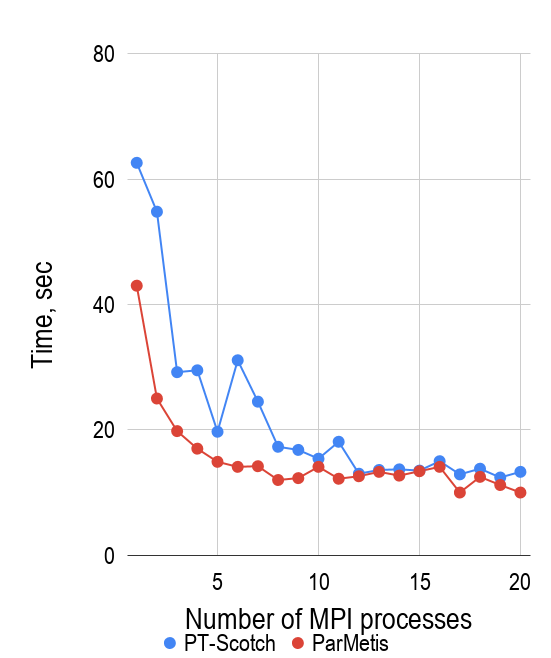
\includegraphics[width=0.48\textwidth]{figures/chapter-2/ordering/k3-18.png}} &
		\subfloat[cube-64]{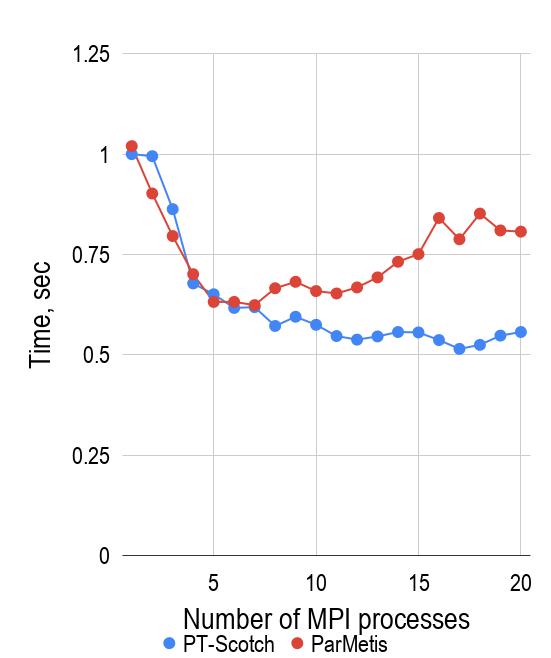
\includegraphics[width=0.48\textwidth]{figures/chapter-2/ordering/cube-64.png}} \\
		\subfloat[pwr-3d]{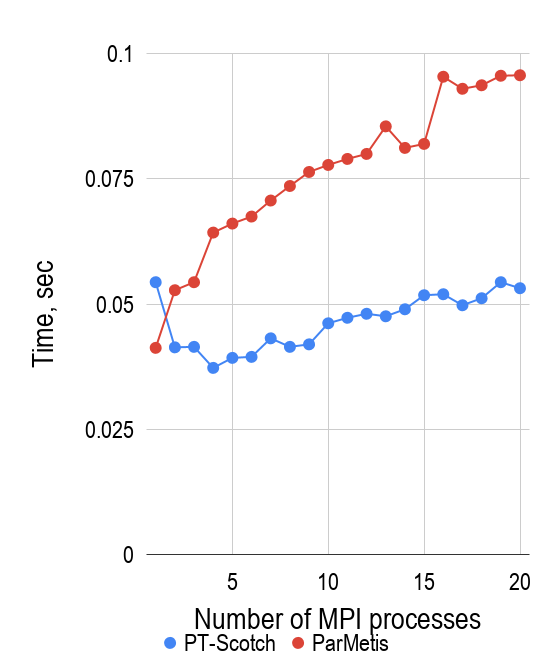
\includegraphics[width=0.48\textwidth]{figures/chapter-2/ordering/pwr-3d.png}} &
		\subfloat[k3-2]{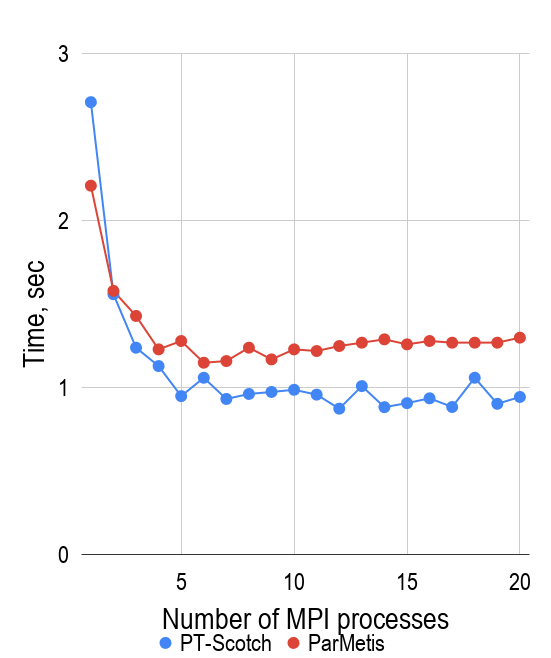
\includegraphics[width=0.48\textwidth]{figures/chapter-2/ordering/k3-2.png}} \\
	\end{tabular}
	\caption{Comparison of different fill-reducing algorithms}
	\label{fig:mumps-ordering-1}
\end{figure}



As the results show, ParMETIS scales much better in contrast to PT-Scotch. In average, the run-time is reduced by approximately BLA \% and BRA \% around the saturation point. Unfortunately, it is difficult for us to give a detailed explanation of the results because there is no access to the assembly tree structure from outside of MUMPS, known to us. Additionally, profiling and tracing of both packages, ParMETIS and PT-Scotch, are required which is out of the scope of this study.\\



\begin{table}[htpb]
\centering
\begin{tabular}{|c|c|c|c|c|}
\hline
Matrix Name & Ordering  & n       & nnz      & nnz / n \\ \hline
cube-5      & PT-Scotch & 9325    & 117897   & 12.6431 \\ \hline
cube-64     & PT-Scotch & 100657  & 1388993  & 13.7993 \\ \hline
cube-645    & ParMetis  & 1000045 & 13906057 & 13.9054 \\ \hline
k3-2        & PT-Scotch & 130101  & 787997   & 6.0568  \\ \hline
k3-18       & ParMetis  & 1155955 & 7204723  & 6.2327  \\ \hline
pwr-3d      & PT-Scotch & 6009    & 32537    & 5.4147  \\ \hline
\end{tabular}
\end{table}


\begin{table}[htpb]
\centering
\begin{tabular}{|c|c|c|c|c|}
\hline
Matrix Name & Ordering  & n       & nnz      & nnz / n \\ \hline
cant        & ParMetis  & 62451   & 4007383  & 64.1684 \\ \hline
consph      & PT-Scotch & 83334   & 6010480  & 72.1252 \\ \hline
memchip     & PT-Scotch & 2707524 & 13343948 & 4.9285  \\ \hline
PFlow\_742  & PT-Scotch & 742793  & 37138461 & 49.9984 \\ \hline
pkustk10    & PT-Scotch & 80676   & 4308984  & 53.4110 \\ \hline
torso3      & ParMetis  & 259156  & 4429042  & 17.0903 \\ \hline
x104        & PT-Scotch & 108384  & 8713602  & 80.3956 \\ \hline
CurlCurl\_3 & PT-Scotch & 1219574 & 13544618 & 11.1060 \\ \hline
Geo\_1438   & xxx       & 1437960 & 63156690 & 43.9210 \\ \hline
nlpkkt80    & xxx       & 1062400 & 28192672 & 26.5368 \\ \hline
\end{tabular}
\end{table}


